
%(BEGIN_QUESTION)
% Copyright 2014, Tony R. Kuphaldt, released under the Creative Commons Attribution License (v 1.0)
% This means you may do almost anything with this work of mine, so long as you give me proper credit

Calculate all listed values for this transformer circuit:

$$\includegraphics[width=15.5cm]{i01257x01.eps}$$

\begin{itemize}
\item{} $V_{primary} = $
\item{} $V_{secondary} = $
\item{} $I_{primary} = $
\item{} $I_{secondary} = $
\end{itemize}

Explain whether this is a {\it step-up}, {\it step-down}, or {\it isolation} transformer, and also explain what distinguishes the ``primary'' winding from the ``secondary'' winding in any transformer.

\vfil 

\underbar{file i01257}
\eject
%(END_QUESTION)





%(BEGIN_ANSWER)

This is a graded question -- no answers or hints given!

%(END_ANSWER)





%(BEGIN_NOTES)

\begin{itemize}
\item{} $V_{primary} = 3.7 \hbox{ volts}$
\item{} $V_{secondary} = 12.0 \hbox{ volts}$
\item{} $I_{primary} = 26.1 \hbox{ mA}$
\item{} $I_{secondary} = 8.02 \hbox{ mA}$
\end{itemize}

This is a {\it step-up} transformer.

%INDEX% Electronics review: transformer ratios

%(END_NOTES)


